\subsubsection{Informazioni sul package}
\begin{figure}[h]
	\centering
	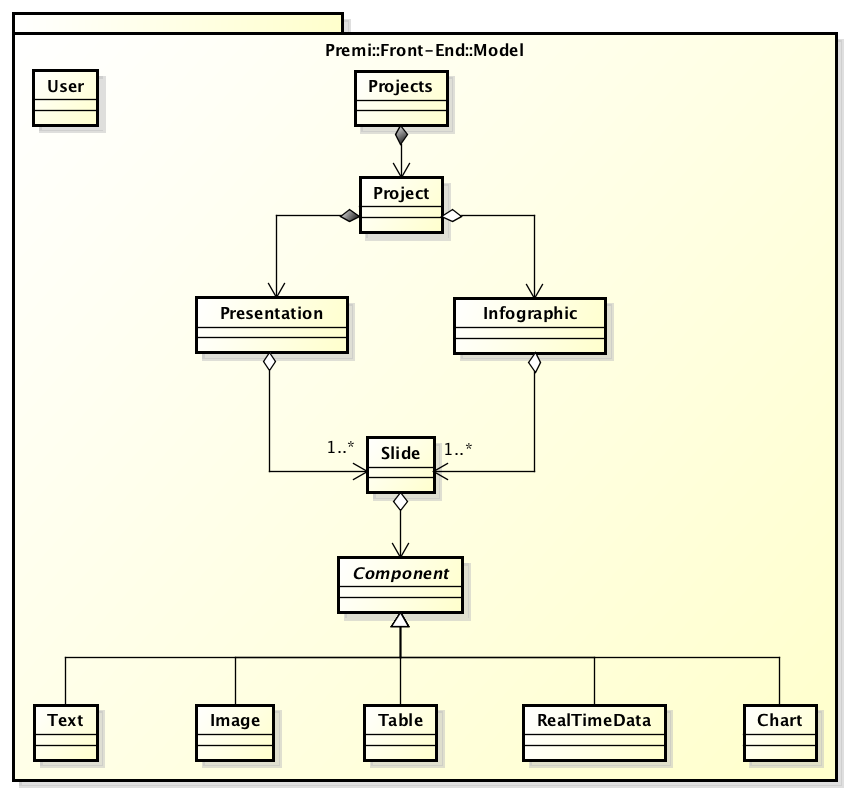
\includegraphics[width=0.9\linewidth]{img/front-end_model}
	\caption[Premi::Front-End::Model]{Premi::Front-End::Model}
\end{figure}
\begin{itemize}
	\item \textbf{Descrizione}: Il package serve per mantenere i dati relativi al \textit{\gls{front-end}} e tutta la loro logica di \gls{business}.
	\item \textbf{Interazione con altri package}:
	\begin{itemize}
		\item Vi è un'interazione con il package Premi::Front-End::Services responsabile del recupero e salvataggio delle informazioni e dell'invocazione di precise procedure dall'esterno mediante chiamate REST;
		\item Vi è un'interazione con il package Premi::Front-End::Controller necessaria per far comunicare il model con le view;
		\item Vi è un'interazione con il package Premi::Front-End::Views necessaria per fornire i dati da far visualizzare all'utente;
		\item Vi è in'interazione con il package Premi::Front-End::Directives responsabile nel collegamento tra le view e i controller del package.
	\end{itemize}
\end{itemize}

\subsubsection{Classi contenute}
\begin{itemize}
	\item Premi::Front-End::Model::Projects:
	\begin{itemize}
		\item \textbf{Descrizione}: classe per la gestione di una collezione di progetti. Un progetto racchiude una presentazione e zero o più infografiche.
		\item \textbf{Relazioni con altre classi}:
		\begin{itemize}
			\item Premi::Front-End::Model::Project.
		\end{itemize}
	\end{itemize}
	\item  Premi::Front-End::Model::Project:
	\begin{itemize}
		\item \textbf{Descrizione}: classe per la gestione di un progetto.
		\item \textbf{Relazioni con altre classi}:
		\begin{itemize}
			\item Premi::Front-End::Model::Presentation;
			\item Premi::Front-End::Model::Infographic.
		\end{itemize}
	\end{itemize}
	\item  Premi::Front-End::Model::Infographic:
	\begin{itemize}
		\item \textbf{Descrizione}: classe per la gestione di una \gls{infografica}. Un'\gls{infografica} ha il compito di raggruppare più \gls{slide} in un \gls{template} grafico scelto dall'utente in un ordine impostabile di volta in volta.
		\item \textbf{Relazioni con altre classi}:
		\begin{itemize}
			\item Premi::Front-End::Model::Slide.
		\end{itemize}
	\end{itemize}
	\item   Premi::Front-End::Model::Presentation:
	\begin{itemize}
		\item \textbf{Descrizione}: classe per la gestione di una presentazione. Una presentazione raggruppa più \gls{slide}. Per la visualizzazione delle presentazioni è stato scelto di utilizzare il \gls{framework} \gls{Reveal.js} che permette di avere una visualizzazione a griglia, di conseguenza una presentazione deve memorizzare anche le coordinate delle sue \gls{slide}.
		\item \textbf{Relazioni con altre classi}:
		\begin{itemize}
			\item Premi::Front-End::Model::Slide.
		\end{itemize}
	\end{itemize}
	\item Premi::Front-End::Model::Slide: Classe per la gestione di una \gls{slide}.
	\begin{itemize}
		\item \textbf{Descrizione}: classe per la gestione di una \gls{slide}.
		\item \textbf{Relazioni con altre classi}:
		\begin{itemize}
			\item Premi::Front-End::Model::Component.
		\end{itemize}
	\end{itemize}
	\item  Premi::Front-End::Model::Component:
	\begin{itemize}
		\item \textbf{Descrizione}: Classe astratta concretizzata ed estesa dalle varie componenti implementando il pattern \textit{composite} per fare si che elementi foglia e collezione vengano trattati allo stesso modo. Nello specifico, una tabella rappresenta un aggregato di altre componenti.
	\end{itemize}
	\item  Premi::Front-End::Model::Text:
	\begin{itemize}
		\item \textbf{Descrizione}: classe per la gestione di un elemento testuale e delle sue proprietà di formattazione. Concretizza ed estende Premi::Front-End::Model::Component.
		\item \textbf{Relazioni con altre classi}:
		\begin{itemize}
			\item Premi::Front-End::Model::Component.
		\end{itemize}
	\end{itemize}
	\item  Premi::Front-End::Model::Image:
	\begin{itemize}
		\item \textbf{Descrizione}: lasse per la gestione di un elemento di tipo immagine.
		\item \textbf{Relazioni con altre classi}:
		\begin{itemize}
			\item Premi::Front-End::Model::Component.
		\end{itemize}
	\end{itemize}
	\item  Premi::Front-End::Model::Table:
	\begin{itemize}
		\item \textbf{Descrizione}: classe per la gestione di una tabella. Una tabella può contenere altre componenti che concretizzano la classe Premi::Front-End::Model::Component.
		\item \textbf{Relazioni con altre classi}:
		\begin{itemize}
			\item Premi::Front-End::Model::Component.
		\end{itemize}
	\end{itemize}
	\item  Premi::Front-End::Model::RealTimeData:
	\begin{itemize}
		\item \textbf{Descrizione}: classe per la gestione di componenti che si aggiornano in tempo reale con cadenza personalizzabile.
		\item \textbf{Relazioni con altre classi}:
		\begin{itemize}
			\item Premi::Front-End::Model::Component.
		\end{itemize}
	\end{itemize}
	\item  Premi::Front-End::Model::Chart:
	\begin{itemize}
		\item \textbf{Descrizione}: classe per la gestione dei dati necessari per disegnare un grafico.
		\item \textbf{Relazioni con altre classi}:
		\begin{itemize}
			\item Premi::Front-End::Model::Component.
		\end{itemize}
	\end{itemize}
	\item  Premi::Front-End::Model::User:
	\begin{itemize}
		\item \textbf{Descrizione}: classe per la gestione degli utenti.
	\end{itemize}

\end{itemize}
